\begin{figure}[!ht]
    \centering
    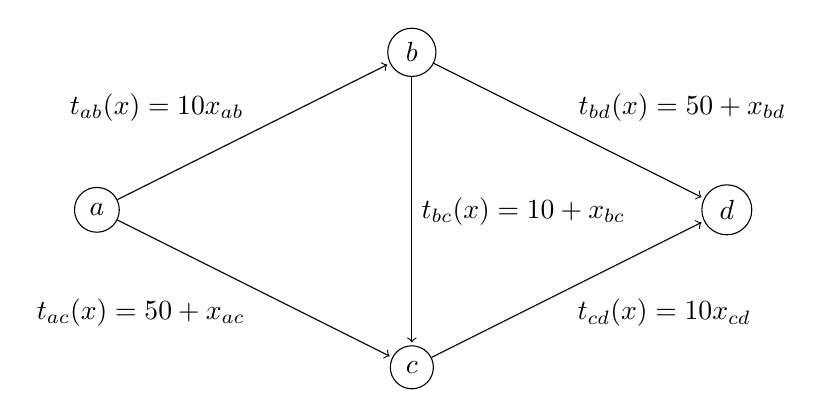
\begin{tikzpicture}[vertex/.style={circle, draw}]
        \node[style=vertex] (a) at (-4, 0)  {$a$};
        \node[style=vertex] (b) at (0, 2)  {$b$};
        \node[style=vertex] (c) at (0, -2) {$c$};
        \node[style=vertex] (d) at (4, 0)  {$d$};
        
        \draw[every loop]
            (a) edge node[above left] {$t_{ab}(x)=10 x_{ab}$} (b)
            (a) edge node[below left] {$t_{ac}(x)=50 + x_{ac}$} (c)
            (b) edge node[above right] {$t_{bd}(x)=50 + x_{bd}$} (d)
            (c) edge node[below right] {$t_{cd}(x)=10 x_{cd}$} (d)
            (b) edge node[right] {$t_{bc}(x)=10+x_{bc}$} (c)
        ;
    \end{tikzpicture}
    \caption{The Braess network. Each link is labeled with the link cost function.}
    \label{fig:braess-network}
\end{figure}